\label{sec:trading}

This demonstration is of an end-to-end algorithmic trading platform showing the
advantages of coupling application and data management logic, in addition to
scaling out data processing. For example, we can use application logic to
coordinate messaging and execute protocols, functionality that traditionally
does not concern data management systems, while still taking advantage of
efficient processing techniques once we have structured data in hand. Our
algorithmic trading platform will provide tools to simulate markets, with the
primary form of data being order books capturing buy and sell orders from market
participants. The platform consists of three high-level components: i) a stock
exchange simulator, ii) a trading platform runtime built on top of the
\compiler\ runtime that executes trading algorithms (algos), and iii) a trading
workstation where users can interactively enter, modify and visualize the
behavior of their algos. We describe these components before discussing the
workflow.

\tinysection{Stock exchange simulator} In order to validate the efficacy of
their algos, many trading firms perform simulations, or backtesting of their
algos in a controlled setting. Our trading platform will include a stock
exchange simulator whose role is to execute a double auction that matches buyers
to sellers placing limit and market orders. Matching occurs on order books,
which are two relations maintained internally within electronic exchanges such
as NASDAQ and NYSE, and include attributes such as an order identifier, security
symbol, price and volume, as seen when adding orders in the NASDAQ
Totalview-ITCH format~\cite{totalview-url}.

While the core matching logic performed by an exchange is well defined, the
underlying challenge is to provide an environment for testing algos that
reflects actual markets as best possible. Trading firms frequently use
historical traces of actual events on markets as test cases, thus our simulator
supports replay functionality, and critically, combines these historical traces
with actions placed by the algos undergoing testing. The use of historical
traces also enables simulation at scale, as opposed to running algos to simulate
the combined behavior of each individual broker trading on the market.

\comment{
\todo{Implementation with which tools?}
\todo{More on merging historical with live orders?}
\todo{Implement Omniscient Trader Methodology (OTM) for comparison purposes?}
\todo{Advanced use of historical data, e.g. level 1: NYSE TAQ?}
\todo{Describe streams: i) input, on which new orders are specified by
clients, ii) output, reflecting changes to order books back to each subscriber.
This allows all other components in the system to maintain a read-only copy of
the order books, with any changes to the order book first sent to the exchange
before being reflected at subscribers' caches.}
}

\tinysection{Trading algorithms}
The goal of our trading platform is to facilitate the simple and rapid
development of trading algorithms. In many trading firms, after teams of
researchers develop prototypes of algorithms, software engineers painstakingly
transform such algorithms into efficient low-level code for deployment on
trading platforms. Our view is that a software stack coupling declarative query
capabilities integrated with general purpose programming will greatly improve
this development cycle.

In this demonstration, we will provide examples of algos implemented using
queries to perform basic analytical computations, encompassed by order routing
logic to submit and be notified of orders occurring at the stock exchange.  In
particular, we will provide a set of predefined indicators on order books, such
as momentum, volatilities, volume and time-weighted average prices (VWAP, TWAP),
order book imbalances (SOBI, NOII), market aggregate order aggressiveness
(MAOA), expressed as and composed with SQL queries. These indicators can then be
used in strategies such as trend following, market-making (placing orders on
both the bid and sells book to profit off the spread), iceberging (breaking up a
large order into smaller orders to lower transaction costs), sniping (placing
market orders in dark pools in increments until completion or a price limit is
met), and sniffing (placing small market orders to determine behaviors of other
algos), amongst many others.
\comment{
\todo{Explain dark pools. Iceberging as a primitive for any large orders placed
by higher-level algos, as an example (iceberg\_order table, joined with bids and
asks, yielding a fractional order)}
}

In addition to analysis of order books, algos maintain a set of orders placed at
the exchange, and communicate with the exchange to reflect modifications to
active orders. Messaging is awkward to perform from a database or stream
processor, and requires an additional software component such as a client or
proxy. Furthermore communication can be complex, for example algos can interact
with multiple exchanges simultaneously as is commonly occurring with the rise of
dark pools and smart order routing processes. Our algos will make use of
\targetlang\ code residing within the same process space as query results to
provide zero-copy communication.

\comment{
\begin{itemize}
  \item Advanced algorithms: combining level I and level II algorithms,
  combining alternate data sources, e.g. news feeds, twitter feeds. Would be
  nice to have learning algorithms and maintenance for them.
  \item Portfolio management.
\end{itemize}

\todo{Tie in with description of how apps and queries interact
on the runtime.}
\todo{Many algos, implemented on top of DBToaster runtime.}
}


\tinysection{Trading workstation}
The trading workstation combines algo development with interaction on an algo's
execution, enabling human monitoring of the active orders placed by an algo as
well as both direct manipulation of the active orders and visualization of the
current state of the market's microstructure (order books and charts displaying
statistics of the order books). The editor supports the development of
\targetlang\ programs consisting of language integrated queries, through which
users may inspect or design algos. These algos are compiled into modules and
submitted to the trading platform runtime. For the visualizer, charting and
graphing components can also take advantage of language integration, using
queries to locally compute the desired statistics on order books. These queries
would be materialized as views by \compiler and kept fresh with the exchange's
output stream, coupling an event-driven visualization with order book update
events.

\begin{figure}[htbp]
\begin{center}
\vspace{-5mm}
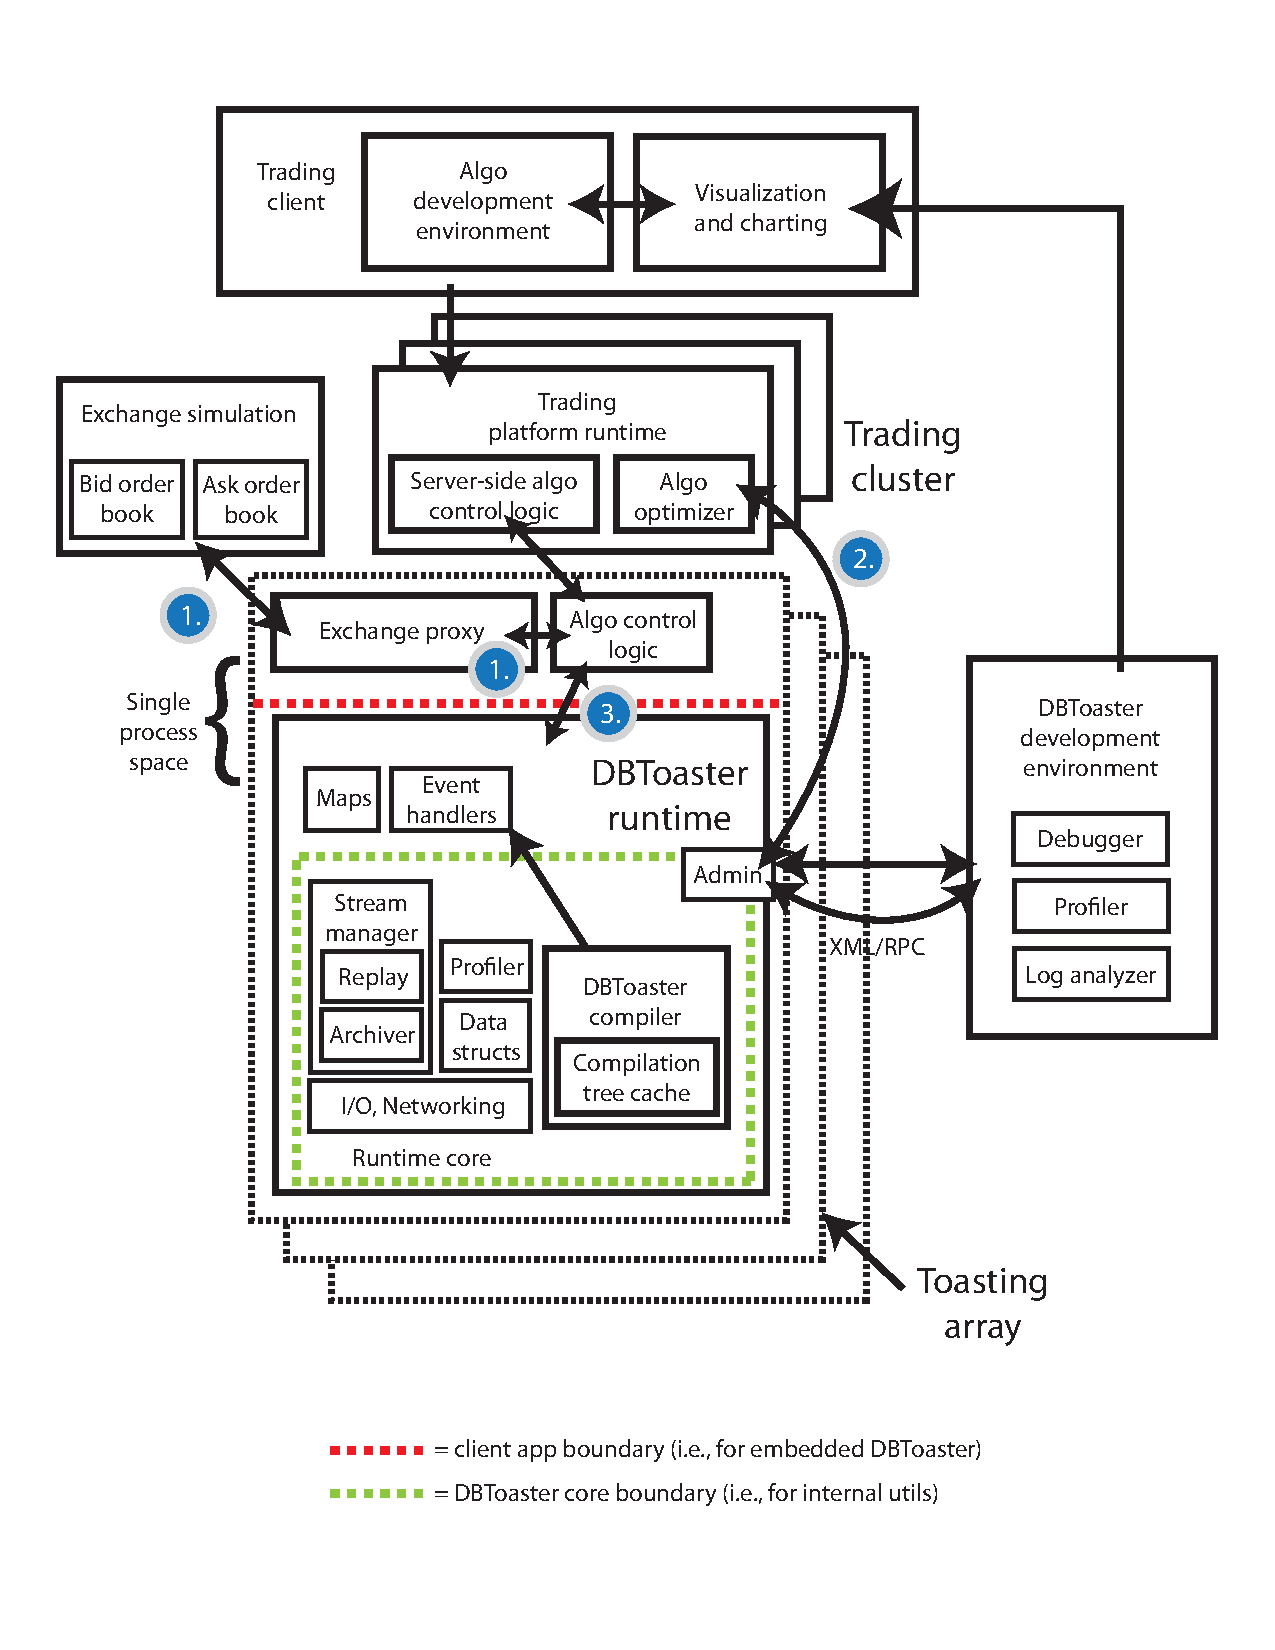
\includegraphics[scale=0.33]{figures/finapp}
\end{center}
\label{fig:algarch}
\vspace{-10mm}
\caption{Algorithmic trading platform design.}
\end{figure}


\tinysection{Algorithmic trading workflow}
Figure~\ref{fig:algarch} is an architecture diagram of our algorithmic trading
platform built on top of the \compiler\ platform. To summarize the workflow
described for the three components above, algo developers and traders use the
trading workstation to submit new algos to the trading platform runtime and
monitor their behavior. The trading platform runtime is the \compiler runtime as
described in Section~\ref{sec:dbtoaster} executing algos compiled into
\targetlang\ operators. In addition to \compiler\ trigger programs maintaining
agile views and query results, these operators may include messaging and control
logic to perform tasks such as smart order routing across multiple exchanges.
The trading platform maintains input streams coming from each exchange in the
system to provide a read-only copy of each exchange's order books. The trading
platform provides output streams to each exchange through which algos can send
order requests and modifications. Finally the stock exchange simulator accepts
new and updates to orders on its input streams, applies a matching process to
enact trading, and reflects the status of the order books to all subscribers. 
